\chapter{Methodology}\label{ch:methodology}

Data Quality methodology consists of two main parts, the model and the metamodel.
The model defines activities, their description, goals and sequence of order needed for extraction of Data Quality metrics.
The metamodel defines components of DQ process, maps the relationship among the components and activities respectively.

\section{Data Quality vs Security}

In addition to model and architecture security mechanism, we have to consider security of data sets.
Data often contains personal information of users - so called \textit{sensitive attributes}.
Such information can be in a~form of personal identifiers or quasi-identifiers.
\textit{Personal identifier} is an unique information that identifies a~user - a~birth number, bank account number and other types of personal IDs.
\textit{Quasi-identifiers} are characteristics which needs to be used in combination with others to identify an entity - examples are gender, postal code, age or nationality.

To prevent data stealing and following re-identification of users, several models exists to protect personal information of individuals in dataset.
Those privacy models are \textbf{optimal k-anonymity}, \textbf{l-diversity}, \textbf{t-closeness} and \textbf{differential privacy}.
Three general types of attack to datasets exists:
\begin{enumerate*}[label=(\roman*)]
    \item \label{itm:reident} re-identifying an individual,
    \item \label{itm:query} query whether an individual is a~member of a~dataset,
    \item \label{itm:linking} linking an individual to a~sensitive attribute.
\end{enumerate*}

\textbf{Optimal k-anonymity} protects against both cases~\ref{itm:reident} and~\ref{itm:query} by transforming quasi-identifiers so that at least \( k - 1 \) members of set are indistinguishable from each other - group based anonymization.
Identifiers are transformed by suppression (needless attributes are replaced with \textit{dummy} values) and generalization (individual values of attributes are replaced with a~broader category - e.g.\ specific age can be replaced by a~range).
As \( k \) increases risk of data exploit reduces, on the other hand data quality decreases - we are talking about a~\textit{privacy-utility} tradeoff.
Moreover, the \( k \) is limit - in order for this method to work if \( k \) is set to \( k \triangleq 10 \) then any group must contain at least \( 10 \) individuals.
The first drawback of k-anonymity is vulnerability to \textit{homogeneity attack} which works on premise of data having sensitive value identical within a~set of \( k \) records - it is enough to find the group of records, the individual belongs to, if all of them have the same sensitive value.
Second drawback is the possibility of \textit{background knowledge attack} where attacker identifies associations among one or more quasi-identifiers and reduces the set of possible values for the sensitive attribute.

Both \textbf{l-diversity} and \textbf{t-closeness} are group based anonymization techniques building on a~concept of \textbf{optimal k-anonymity}.
In addition to \textbf{optimal k-anonymity}, \textbf{T-closeness} transforms quasi-identifiers such that each group is within a~distance \( t \) of the distribution of sensitive values for the entire dataset~\cite{web:privacy-models}.
The distance is measured as the cumulative absolute difference of the distributions, as \( t \) decreases both risk of sensitive attribute disclosure and data quality decreases.
Suppose that the sensitive attribute is salary.
Each group's frequency distribution of salary will be within a~distance \( t \) from the salary frequency distribution for the entire dataset~\cite{web:privacy-models}.

\textbf{Differential privacy} and its variants (epsilon, epsilon-delta) are statistical techniques aiming to protect data against \textit{differentiated attack}.
The model guarantees that even if someone has complete information about 99 of 100 people in a~data set, they still cannot deduce the sensitive information about the final person~\cite{web:differential-privacy}.
The mechanism works by adding random noise to the aggregate data, leaving only a~trend without possibility to figure out exact values in data (e.g.\ information that \( n\% \) of users prefer some product over another).

\section{Business Problems and Data Defects}

TODO

\section{Model}

The methodology has several important components that need to be identified or developed.
The metamodel that covers the required components is as depicted in figure~\ref{fig:methodology-metamodel}.
The activities within the process model have a goal to develop those components.

Overall, the methodology consists of two main processes.
The first one is \textbf{Specification Process}.
The goal of this processs is to identify and define context specific ways to measure data quality.
The second one is an \textbf{Execution Process}.
Its main goal is to \textit{collect} and \textit{verify} data with output from \textit{Specification Process} taken into account.

\begin{figure}[htb]
    \centering
    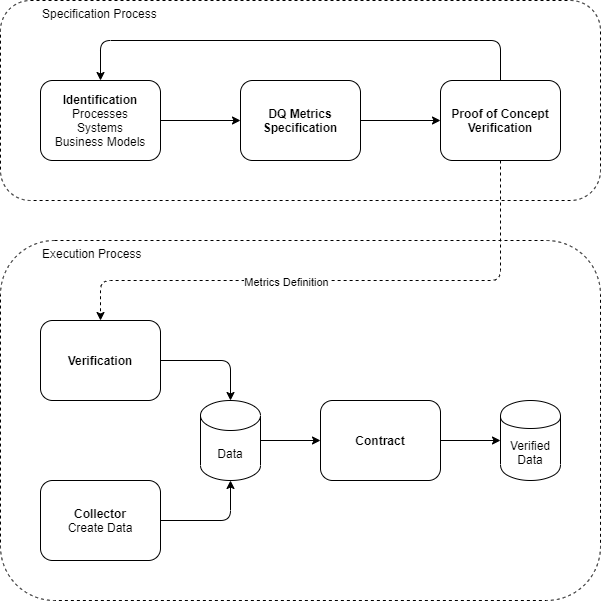
\includegraphics[width=0.7\textwidth]{figures/dq-methodology.png}
    \caption{Methodology Metamodel}
    \label{fig:methodology-metamodel}
\end{figure}
\FloatBarrier

\subsection{Specification Process}

TODO

\subsubsection{Identification}

This activity focuses on identification of systems, processes and business schemes generatig data.
By identifying weak points and bottlenecks in those processes, we can find causes of poor data.
Also, we need to identify the subprocesses or activities that are mostly affected by the product data quality.

\subsubsection{Metrics Specification}

The goal of this activity is to identify the process metrics or KPIs.
Measuring data quality is all about understanding what data quality attributes are and choosing the correct data quality metrics.
Data Quality Attributes were discussed in back in chapter~\ref{ch:literature-review} section~\ref{sec:data-quality-attributes} and will be further discussed in chapter~\ref{ch:quality-classification-system}.

\subsubsection{Proof of Concept Verification}

The last part of current process is verification and Proof of Concept.
This activity has to ensure that selected metrics are meaningful enough, capturing the actual condition of data.

\subsection{Execution Process}

TODO

\subsubsection{Collection}

Data collection is a systematic process of gathering observations or measurements.
Data collector can be either \textit{Information System}, computer program or a human.
Before the beginning of collecting data, we need to consider:

\begin{itemize}
    \item the type of data we will collect;
    \item the methods and procedures we will use to collect, store and process data.
\end{itemize}

\subsubsection{Verification}

In our general case, verification is based on actual reliability of data, computed using DQ metrics.
In other scenarios, the verification could be based on data redundancies, therefore based on the comparison of the collected data from two or more different collectors.
If all data match, the data will be considered as valid.
If not, the data remains invalid until a further collector validates it.

Artificial Intelligence and Machine Learning could be used to further ease and optimize data verification.
Especially when processing image data and data with a high level of abstraction.

\subsubsection{Contract}

TODO

\subsection{Supporting Techniques}

TODO

\subsubsection{Proof of Constancy}

Proof of Constant Data, alias Proof of Constancy, is a way to assure a constant accuracy of data.
Data have to be regularly updated to keep the accuracy rate high.
Data accuracy rate will decrease progressively based on a specific time frame basis (e.g., X\% per month).
This percentage is different depending on the type of data.
Data sets more sensitive to changes may see this rate decrease by 5\% to 10\% per month or day depending on the circumstances.
On the other hand, established, well-known sets, will see their rate decrease by 0.1\% per month or even year.
A scale of discount rates will have to be established based on the areas of interest and actual items collected.

\subsubsection{Proof of Trust}

Proof of Trust is an instrument for data collector evaluation.
The collector or generator will get \enquote*{quality score} for his/her or its collection actions.
The more collectors initiate, update and verify data correctly, the higher their \enquote*{quality score} will be.
A higher quality score leads to a higher level of \enquote*{trust}.
On the other hand, incorrect collection leads to a retroactive decrease of the collector's quality score.

\subsection{Roles}

TODO

\section{Use Cases}

In this part, we will present several use cases, to illustrate versatile use of the presented framework.

\subsection{Enterprise Information System}

Enterprises suffer from poor data quality.
We propose, following the methodology, to introduce a central register of data sources.
This central register should be supported by a set of services and a central data repository.

After a thorough analysis of data requirements and their quality, a defined set of metrics and key performance indicators parameterizes the verification chain of activities.
If the predefined quality limit is not met, the data will either be rejected or saved with an error flag.
% Jestliže data splňují požadovanou úrověň chybovosti, projdou kontraktačním procesem a jsou požadována za referenční až do doby, kdy je jejich poslední verze je nařazeným procesem kvalitativně degradována a označena za nedůvěryhodnou.
If the data meets the required level of error, they go through the contracting process and are considered as a reference until their latest version is qualitatively degraded by the ordered process (e.g., Proof of Constancy) and marked as untrusted.

% Penalizací za špatnou kvalitu by bylo automatické hlášení vyššímu managementu společnosti.
A penalty for poor quality would be automatic reporting to the company's senior management.
% Management by následně mohl uvalit na osoby zodpovědné za konkrétní datové sady a datové toky sankce ve formě snížení nebo zrušení osobních odměn.
Management could then impose sanctions on those responsible for specific datasets and data flows in the form of reductions or cancellations of personal rewards.

\subsection{IoT Cluster}

Based on the domain and usage of the IoT devices, the data repository could be either centralized (e.g., nuclear power plant cluster of secondary senzors) or decentralized (e.g., community weather stations).

The verification algorithm would - in this case - consist from two general authorities.
The first authority being \textit{k} nearest neighbours of the same sensors (or IoT devices in general), and the second one being the set of domain rules.
Nearest neighbors provide redundancy by which data can be verified.
A data samotná musí samozřejmě splňovat kriteriální omezení daná doménou využití.

% Špatnou kvalita by vedla ke snížení významnosti senzoru v klusteru, případně jeho dočasnému nebo úplnému vyřazení z provozu.
Poor quality would reduce the importance of the sensor in the cluster, or its temporary or complete decommissioning.
% Tento systém by vytořil i velice účinnou obranou bariéru proti útokům.
This system would also create a very effective defense barrier against attacks, especially against data poisoning.

Data poisoning is a class of attacks on machine learning algorithm where an adversary alters a fraction of the training data in order to impair the intended function of the system.
Objective can be to degrade the overall accuracy of the trained classifier, escaping security detection or to favor one product over the another.
Machine Learning systems are usually retrained after deployment to adapt to changes in input distribution, so data poisoning represents serious danger.

Qualitative degradation of data by Proof of Constancy would not be the so important, because we expect very high update frequency.
However, lower update frequancy of IoT device would suggest an error within a system, which could serve as a warning to network operators about a faulty device.
Data from defective equipment should also not be taken into account in many cases.

\subsection{Open Source Data Library}

The last Use Case shows usage of completely decentralized solution.
The system would allow those who collect and generate data to be rewarded and data would be accessible for use within a decentralized marketplace.

